\section{Iniciar sesión}

\begin{figure}[ht]
\centering
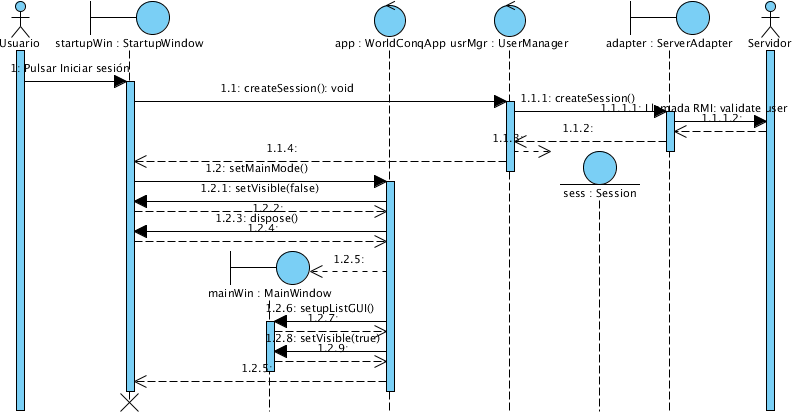
\includegraphics[scale=0.6]{img/ch03devel-login.png}
\caption{Diagrama de secuencia de ``Iniciar sesión''}
\end{figure}

Una vez que el usuario haya introducido sus credenciales, la ventana
\texttt{StartupWindow} pedirá al gestor de usuarios que inicie una nueva
sesión. El gestor de usuarios realizará la llamada RMI a través del
\texttt{ServerAdapter}.

Si los datos son correctos, el servidor devolverá un identificador de sesión.
Con este identificador y el propio nombre de usuario, el gestor de usuarios
creará un nuevo objeto de tipo \texttt{Session}.

A continuación, la ventana \texttt{StartupWindow} pedirá a la clase
\texttt{WorldConqApp} el cambio al modo principal. Al realizar este cambio, se
ocultará la ventana de inicio y se creará la nueva ventana principal
\texttt{Mainwindow}.
